\chapter*{Preface}
We shall start this course with realizing and internalizing a deep and profound truth that will follow us through our coding life and have an important impact on all our projects:

\begin{defbox}[Our Mantra]
\begin{center}
\begin{Huge}
	\emph{Computers are friggin stupid.}
\end{Huge}
\end{center}
\end{defbox}

In principle, this is well and good. If this statement would not hold, we'd have a really hard time making computers do the tasks that are too tedious for us. However, anyone who has ever tried to delegate a part of their chores to a less gifted contemporary knows how \emph{on point} the instructions for their coeval have to be. For computers, this is even only more so. In the tutorials, I've often heard the participants say things like \emph{I thought, the computer would understand that ...}, which I like to acquit with \emph{You think -- the computer does not.}

In this course, I want to guide you through both, the concepts according to which a computer works and the thought processes that you as a programmer should devellop to translate your real life goals into code. In particular, we will be learning the specifics of the programming language C. This language which first appeared in ancient times\footnote{\ie in 1972} has been expanded upon ever since and influenced virtually all modern languages such as C++, C\#, Java, Python, Rust, Go, Perl, Julia, ... You may think of this course as a general introduction to programming. If you ever get to learn another programming language, you will recognize most if not all the concepts discussed here.

This course is aimed at beginners. We will cover all relevant concepts from ground up. I try to keep things interesting while guiding you through the technical details; unfortunately, there are a bunch of them. That means I'll have to ask you to be patient. It will take us a while before we can do anything \emph{interesting} with our programs. However I firmly believe that being able to do things \emph{right} is more rewarding that being able to do things \emph{quickly}\footnote{at least if you can have only either of them.}. To make sure you understand correctly, I'll be providing lots of examples.

While I'll do my best to explain what works how and why, there's no way around doing exercises on your own. I will provide a number of quizz questions at the end of each chapter that are designed to solidify and deepen your understanding of code. Of course, you'll also find solutions in the appendix. Still, I want to encourage you to do your own experiments, be it small code snippets to try your intuition or exercises from external sources. In the end, coding is a skill you can only properly learn by doing.

I should also make clear at the very beginning that programming (in any language) means \emph{applied maths}. While you do not need to have majored maths in university, neither should you have an aversion against tinkering with formulae anf formal logic. A machine that was built to \emph{compute} can only be told what to do using the tools provided by maths.

Note also that this is an introductory course, not a complete reference of all aspects of the C programming language. As a such, I recommend the website \url{cppreference.com}, which does a good job listing all features and expected behaviours. In fact, since I regard this website an essential tool in programming, a short chapter will be dedicated to how to find your way in that encyclopedia.

To go through this course, you will need a current installation of the \emph{Gnu Compiler Collection} (GCC) as well as a simple code editor on your machine. You should find a guide for how to do so on the website where you found this book, as well as alternative options. Further, you should be (superficially) familiar with using the console for invoking programs. While there are other ways of compiling code, I will show exclusively how to do so from the command line. The reason behind this is that I feel in no way capable of treating the myriad of IDEs\footnote{\emph{Integrated Development Environment}; graphical programs that help with writing code.} available ot there, nor the differences that come with the versions written for different operating systems. The somewhat antiquated command line interface, on the other hand, is way more uniform between various machines. Last but not least, you can derive the correct handling of your IDE from understanding the command line; an IDE is only a \emph{frontend} to the command line interface, \ie it will generate the same commands that I shall show you here.

Since this approach means we are dealing with two different environments -- the command line and our C code -- it is only reasonable to reflect this fact graphically in this book. In- and Output on the command line will be rendered in black boxes like the following:
\begin{cmdbox}[Command Line Interface]
\texttt{{\color{green}blue-chameleon@blue-chameleon-HP-250-G8-Notebook-PC}:{\color{blue!80!white}\textasciitilde}\$ cd Codes} \\
\texttt{{\color{green}blue-chameleon@blue-chameleon-HP-250-G8-Notebook-PC}:{\color{blue!80!white}\textasciitilde\textbackslash Codes}\$}
\end{cmdbox}

More often than not, the preface to the command line interface (the green and blue text) will be omitted, and only the commands themselves as well as their output are presented. To distinguish between commands and output, the former will be prefaced with a Dollar sign (\texttt{\$}):

\begin{cmdbox}[Command Line Interface]
\texttt{\$ echo hello world} \\
\texttt{hello world}
\end{cmdbox}

C-Code, on the other hand, will be rendered in white boxes with \emph{syntax highlighted}\footnote{To make code easier readable for humans, it is custom to render the various parts in different colours. Syntax highlighting means applying these rules for colouring.} code together with line numbers:
\begin{codebox}[helloworld.c]
\begin{minted}[linenos]{c}
#include <stdio.h>

int main () {
    printf("hello world\n");
}
\end{minted}
\end{codebox}

Where relevant, I will also provide the output generated by a program after compiling and executing it. The invocation of the compiler and the compiled program itself will be discussed in the first chapter and omitted thereafter, unless something \enquote{non-standard} is going on.

A picture says more than a thousand words. Where possible, I will provide sketches to illustrate the key concepts of the current discussion. To make them even easier to find when skimming through the book, these schematics are highlighted in a sky blue box. These sketches will be enumerated and listed in the list of figures at the very end of this book. The same type of boxes is used at the end of each chapter to summarize the main takeaways.

\begin{defbox}[Path to Success]
\begin{center}
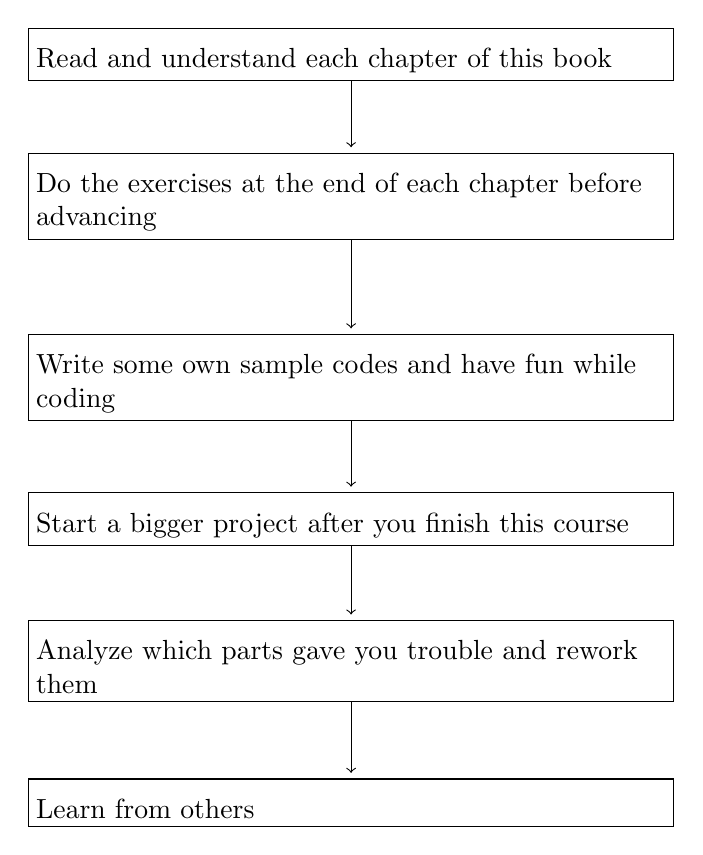
\begin{tikzpicture}
  [
    cell/.style={text width=80mm,
      text height=4mm, draw=black, inner sep=1mm},
    ld/.style={draw=black,shorten >=2pt,->}
  ]
  \node (c1) at (0,9.5) [cell] {Read and understand each chapter of this book};
  \node (c2) at (0,7.7) [cell] {Do the exercises at the end of each chapter before advancing};
  \node (c3) at (0,5.4) [cell] {Write some own sample codes and have fun while coding};
  \node (c4) at (0,3.6) [cell] {Start a bigger project after you finish this course};
  \node (c5) at (0,1.8) [cell] {Analyze which parts gave you trouble and rework them};
  \node (c6) at (0,0.0) [cell] {Learn from others};

  \draw [ld] (c1.south) -> (c2.north);
  \draw [ld] (c2.south) -> (c3.north);
  \draw [ld] (c3.south) -> (c4.north);
  \draw [ld] (c4.south) -> (c5.north);
  \draw [ld] (c5.south) -> (c6.north);
\end{tikzpicture}
\end{center}
\end{defbox}

Some text will be set off the principal text in a box with a grean headline. The content of these boxes is a tangent to what the full text tries to explain and will often contain good pieces of advice or clarifications. You should see them as part of the continuous text that is highlighted to easier find it later on.

\begin{hintbox}[List of Terms]
This book probably will introduce a lot of new concepts to you. If you've forgotten what a certain term means or where to find it, you can look at appendix A. There you'll find an alphabetical list of the concepts and terms introduced in this book.
\end{hintbox}

\emph{errare humanum est} -- and you presumably are a human. Don't worry, I've got you covered. To warn you about situations most beginners (and sometimes even professionals) struggle with, I put boxes with red headlines that show you situations you should avoid, or code that contains a non-obvious error.

\begin{warnbox}[Do not learn all of this by heart]
A good programmer does not necessarily know \emph{all} the details shown in this book. It is sufficient to broadly know about concepts and look up the details when the need arises. Don't bother yourself with memorizing tables that you can look up online or in this book whenever you need to. You will automatically retain the truly important bits simply by repeatedly applying them. Rather, spend your energy on understanding, and doing experiments on your own!
\end{warnbox}

Some of the content is certainly interesting, but maybe less so for absolute beginners; at the very least, those sections are not essential for every day coding. Depending on your level and time restraints, you may want to do a deep dive or cut to the chase. To faciliate this, more advanced content is highlighted in a similar manner:
\begin{plusbox}
In assembly, the hello world program expands to
\begin{codebox}[helloworld.s]
\begin{minted}[linenos]{asm}
        .file   "helloworld.c"
        .text
        .section        .rodata.str1.1,"aMS",@progbits,1
.LC0:
        .string "hello world\n"
        .section        .text.startup,"ax",@progbits
        .p2align 4
        .globl  main
        .type   main, @function
main:
.LFB12:
        .cfi_startproc
        endbr64
        subq    $8, %rsp
        .cfi_def_cfa_offset 16
        leaq    .LC0(%rip), %rsi
        movl    $1, %edi
        xorl    %eax, %eax
        call    __printf_chk@PLT
        xorl    %eax, %eax
        addq    $8, %rsp
        .cfi_def_cfa_offset 8
        ret
        .cfi_endproc
.LFE12:
        ...
\end{minted}
%$
\end{codebox}
\end{plusbox}

This book is based on a university level course for which I was responsible from 2018 through 2022. The experience with different kinds of students and their learning styles have informed the course design in numerous ways. However, time constraints have always curbed my ambitions, and I'm thrilled to expand on my prior work. Ultimatively, of course, this is a piece of human work, and therefore likely to be flawed. I put a lot of effort into the totality of this project, but I can almost guarantee you that you can find at least some minor mistakes. If you do so, or have any questions or remarks on the provided material, feel free to contact me: \url{bluechameleoncoding@gmx.net}

Without further ado, let's start coding!
\begin{flushright}
\myName, \myVersionTime
\end{flushright}